\section{General setup}\label{sec:general-setup}
GRATiS uses GROOVE as a replacement of the IOSTS in ATM. Figure~\ref{fig:tooling} shows the collaboration diagram of GRATiS. GROOVE has several exploration strategies for exploring a GG to a GTS. The SymbolicStrategy is added as exploration strategy. It contains functionality to build an STS from a GG. The STS is sent as a JSON message by the GrooveInterface to a remote host. The ATMInterface receives the message and starts the test run.

\begin{figure}[ht]
  \begin{center}
    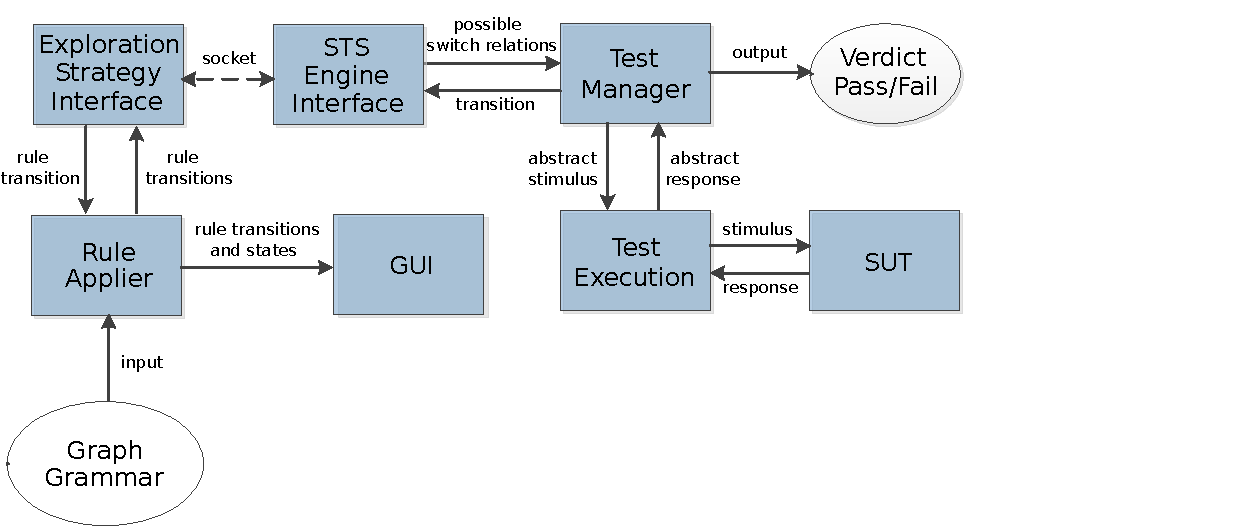
\includegraphics[width=\textwidth]{tooling.pdf}
  \end{center}
  \caption{GRATiS collaboration diagram}
  \label{fig:tooling}
\end{figure}


\section{Description of added functionality}
This section covers in detail the added functionality to GROOVE and ATM. 

\subsection{GROOVE exploration strategy}
Figure~\ref{fig:esi-diagram} shows the class diagram of the added exploration strategy interface. The symbolic exploration strategy has an exploration strategy such as the Breadth-First exploration strategy to explore the GTS. The remote exploration strategy extends the symbolic exploration strategy.

The user starts the remote exploration strategy. This strategy starts a Breadth-First exploration strategy. This strategy explores the GTS and notifies the remote strategy when there are no more rule transitions to explore. The symbolic strategy builds the STS in Java objects using the explored rule transitions. The class diagram  of the STS is given in section~\ref{sec:sts-setup}. The remote strategy sends the STS in JSON format as a HTTP PUT request to the interface at ATM.

The Breadth-First exploration strategy and the symbolic strategy are loosely coupled, such that other strategies can also be used if desired.
 
\begin{figure}[ht]
  \begin{center}
    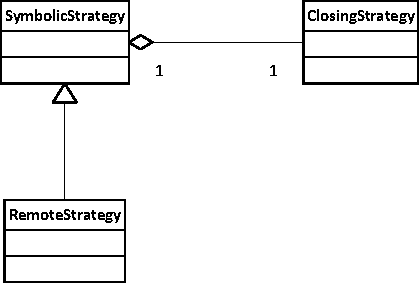
\includegraphics[width=0.35\textwidth]{strategy.pdf}
  \end{center}
  \caption{The class diagram of the exploration strategy interface}
  \label{fig:esi-diagram}
\end{figure}

\subsection{STS}\label{sec:sts-setup}
Figure~\ref{fig:sts-diagram} shows the class diagram of the STS in GRATiS. The STS is composed of Locations, Switch relations, Gates, Interaction and Location variables. A Location can be the start and targent of any number of switch relations. A switch relation has two locations; the start and target location. A Switch relation has one gate and a gate can belong to any number of switch relations. A gate can have any number of interaction variables, but an interaction variable belongs to one gate. The STS has a singleton class, the RuleInspector, which contains the functionality of building guards and updates from rule graphs.

\begin{figure}[ht]
  \begin{center}
    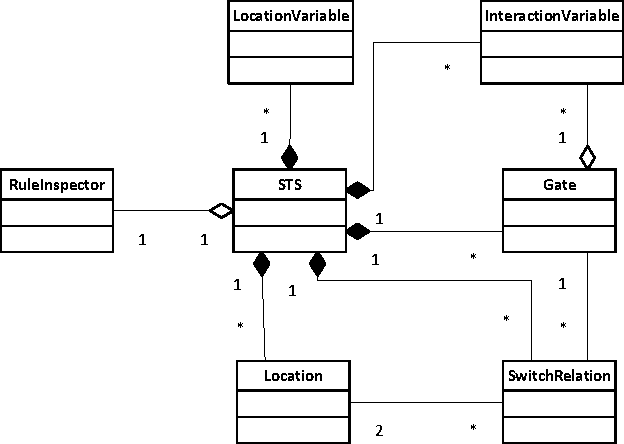
\includegraphics[width=0.5\textwidth]{STS.pdf}
  \end{center}
  \caption{The class diagram of the STS in GRATiS}
  \label{fig:sts-diagram}
\end{figure}

\subsection{ATM Interface}
The ATM interface is one component in the Rails framework. It receives the STS request, builds the STS as Ruby objects and initiates the test run using this STS as model.

\section{Rule priority}
This section covers a specific implementation issue of setting rule priorities in GROOVE.

There can be several outgoing rule transitions from a graph. In GROOVE, rules can have different priority levels. A rule transition with a higher priority rule is explored before rule transitions with lower priority rules. Consider the graph grammar in Figure~\ref{fig:priority_gg}. The 'add' rule produces a rule transition to a graph, where the $sub$ rule produces a rule transition back to the start graph. The 'sub' rule does not match the start graph, because it has a lower priority than the $add$ rule.

\begin{figure}[ht]
  \begin{center}
    \subfloat[The initial graph]{\label{fig:priority_start}% To use this figure in your LaTeX document
% import the package groove/resources/groove2tikz.sty
%
% Special colors
\begin{tikzpicture}[
% Special color styles
scale=\tikzscale]
\node[node] (n1)  at (0.870, -0.680) {\ml{x = 0}};
\userdefinedmacro
\end{tikzpicture}
\renewcommand{\userdefinedmacro}{\relax}
}\hspace{20px}
    \subfloat[The $sub$ rule with priority 0]{\label{fig:priority_sub}% To use this figure in your LaTeX document
% import the package groove/resources/groove2tikz.sty
%
% Special colors
\begin{tikzpicture}[
% Special color styles
scale=\tikzscale]
\node[node, prod] (n4)  at (1.450, -0.990) {\ml{$\pi$1 = 10}};
\node[node, attr] (n6)  at (1.450, -0.410) {\ml{\textbf{int}}};
\node[node, prod] (n7)  at (0.610, -1.660) {\ml{$\pi$1 = 10\\gt = true}};
\node[node, attr] (n8)  at (0.600, -1.000) {\ml{\textbf{int}}};
\node[node] (n9)  at (0.600, -0.400){};
\path[deledge](n9.south -| 0.600, -1.000) -- node[dellab]{x} (n8) ;
\path[edge] (n7)  -- node[lab]{$\pi$0} (n8) ;
\path[newedge](n9.east |- 1.450, -0.410) -- node[newlab]{x} (n6) ;
\path[edge] (n4)  -- node[lab]{$\pi$0} (n8) ;
\path[edge] (n4)  -- node[lab]{sub} (n6) ;
\userdefinedmacro
\end{tikzpicture}
\renewcommand{\userdefinedmacro}{\relax}
}\hspace{20px}
    \subfloat[The $add$ rule with priority 1]{\label{fig:priority_add}% To use this figure in your LaTeX document
% import the package groove/resources/groove2tikz.sty
%
% Special colors
\begin{tikzpicture}[
% Special color styles
scale=\tikzscale]
\node[node] (n0)  at (0.540, -0.560){};
\node[node, attr] (n1)  at (0.540, -1.160) {\ml{\textbf{int}}};
\node[node, prod] (n2)  at (0.550, -1.820) {\ml{$\pi$1 = 30\\lt = true}};
\node[node, attr] (n6)  at (1.390, -0.570) {\ml{\textbf{int}}};
\node[node, prod] (n7)  at (1.390, -1.150) {\ml{$\pi$1 = 10}};
\path[deledge](n0.south -| 0.540, -1.160) -- node[dellab]{x} (n1) ;
\path[edge] (n2)  -- node[lab]{$\pi$0} (n1) ;
\path[newedge](n0.east |- 1.390, -0.570) -- node[newlab]{x} (n6) ;
\path[edge] (n7)  -- node[lab]{$\pi$0} (n1) ;
\path[edge] (n7)  -- node[lab]{add} (n6) ;
\userdefinedmacro
\end{tikzpicture}
\renewcommand{\userdefinedmacro}{\relax}
}
  \end{center}
  \caption{Priority rules}
  \label{fig:priority_gg}
\end{figure} 

The graphs are isomorphic under the point algebra, so they represent the same location. The STS of transforming this graph grammar is in Figure~\ref{fig:priority_sts_wrong}, with $\imath = \{x \mapsto 25\}$. This STS is wrong, because the 'sub' switch relation can be taken from the start.

\begin{figure}[ht]
  \begin{center}
    $\xymatrix{
   \ovalbox{$l_0$} \ar@(ul,ur)[]^{?sub\,|\,x\,>\,10\,|\,x\,:=\,x\,-\,10} \ar@(dl,dr)[]_{?add\,|\,x\,<\,30\,|\,x\,:=\,x\,+\,10}
}$

  \end{center}
  \caption{A wrong STS transformation of the graph grammar in Figure~\ref{fig:priority_gg}}
  \label{fig:priority_sts_wrong}
\end{figure}

The solution is shown in Figure~\ref{fig:priority_sts_right}. The negated guard of the 'add' switch relation is added to the 'sub' switch relation. The optimized guard for this switch relation is 'x >= 30' of course, but this shows the main principle: for each outgoing switch relation, the negated guard of all switch relations represented by higher priority rules must be added to the guard. So, the 'x < 30' guard is negated to '!(x < 30)' and added to yield the 'x > 10 \&\& !(x < 30)' guard. Note that if the 'add' switch relation had no guard, it would be applicable on all graph states with isomorphic abstractions. Therefore, the 'sub' switch relation would not exist, because the 'add' rule is always applicable whenever the 'sub' rule also is.

\begin{figure}[ht]
  \begin{center}
    $\xymatrix{
   \fbox{$l_0$} \ar@(ul,ur)[]_{sub | x > 10 \&\& !(x < 30) | x := x - 10} \ar@(dl,dr)[]_{add | x < 30 | x := x + 10}
}$

  \end{center}
  \caption{A correct STS transformation of the graph grammar in Figure~\ref{fig:priority_gg}}
  \label{fig:priority_sts_right}
\end{figure}
